
\chapter{Introducción específica} % Main chapter title

\label{Chapter2}

%----------------------------------------------------------------------------------------
%	SECTION 1
%----------------------------------------------------------------------------------------
Esta sección presenta una breve introducción técnica a las herramientas hardware y software utilizadas en el trabajo.

\section{Tecnologías de hardware utilizadas}

\subsection{Espressif ESP32}


ESP32 \cite{ESP32} es una serie de microcontroladores embebidos en un chip con Wi-Fi y Bluetooth integrados, de bajo costo y consumo, desarrollado por \textit{Espressif Systems}. Emplea dos cores Xtensa® 32-bit LX6 CPU, incluye interruptores de antena, amplificador de potencia, amplificador de recepción de bajo ruido, un co-procesador ULP (\textit{Ultra Low Power}), módulos de administración de energía y varios periféricos.
En la siguiente imagen (\ref{fig:esp32}) se puede apreciar la placa ESP32-WROOM-32D \cite{ESP32_wroom_32d_datasheet} utilizada para el desarrollo del presente trabajo.

\begin{center}
   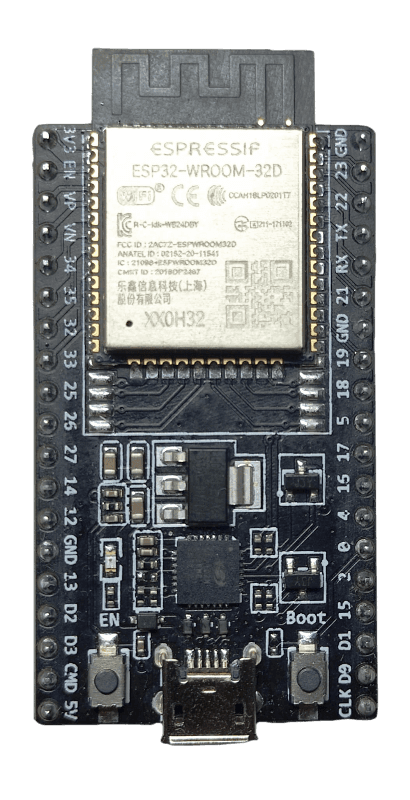
\includegraphics[scale=0.15]{electronics/esp32_2}
   \captionof{figure}{Microcontrolador ESP32-WROOM-32D.}
   \label{fig:esp32}
\end{center}


\subsection{Sensor de temperatura y humedad DHT11}

El DHT11 \cite{DHT11_datasheet} es un sensor digital de temperatura y humedad relativa de bajo costo y fácil uso. Integra un sensor capacitivo de humedad y un termistor para medir el aire circundante, y muestra los datos mediante una señal digital en el pin de datos (no posee salida analógica). Entre otras aplicaciones se lo suele utilizar principalmente en aplicaciones relacionadas al control automático de temperatura, aire acondicionado y monitoreo ambiental en agricultura. En la figura \ref{fig:dht11} se puede apreciar una imagen del componente.

\begin{center}
   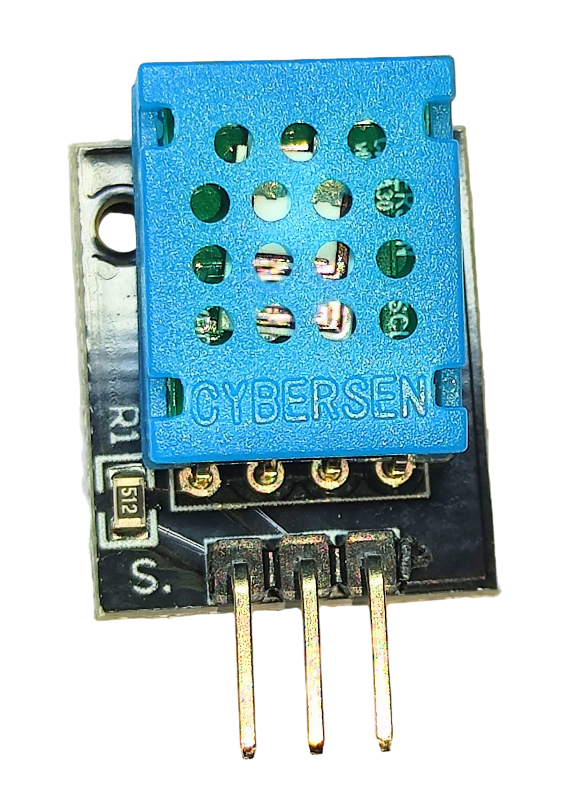
\includegraphics[scale=0.1]{electronics/dht11_2}
   \captionof{figure}{Sensor DHT11.}
   \label{fig:dht11}
\end{center}

\subsection{Sensor de presión BMP280}

El BMP280 \cite{BMP280_datasheet} es un sensor de presión barométrica absoluta, especialmente factible para aplicaciones móviles que puede ser utilizado con I2C o SPI. Permite alta precisión y linealidad, estabilidad a largo plazo, alta robustez a un muy bajo consumo. En la figura \ref{fig:bmp280} se puede apreciar una imagen del componente.

\begin{center}
   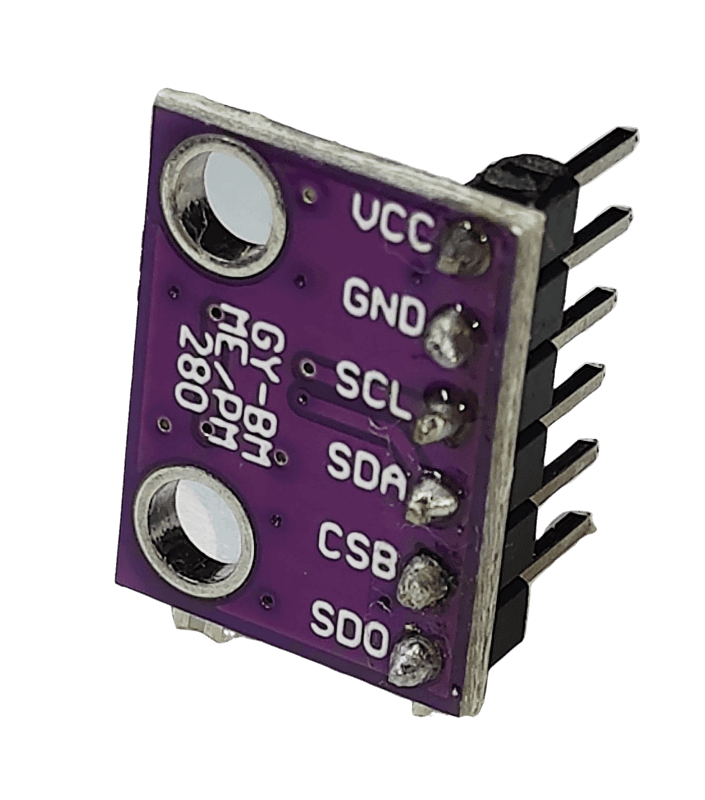
\includegraphics[scale=0.10]{electronics/bmp280_2}
   \captionof{figure}{Sensor BMP280.}
   \label{fig:bmp280}
\end{center}

\subsection{Fotorresistor como sensor de luminosidad}

El fotorresistor es una resistencia eléctrica que varía su valor en función de la cantidad de luz que incide sobre su superficie.
Cuando el fotorresistor no está expuesto a radiaciones luminosas, los electrones están firmemente unidos en los átomos que lo conforman, por lo que alcanza su máxima resistencia eléctrica, y cuando sobre él inciden radiaciones luminosas, esta energía libera los electrones con lo cual el material se vuelve más conductor, y se disminuye su resistencia. En la figura \ref{fig:fotoresistor} se puede apreciar una imagen del componente.

\begin{center}
   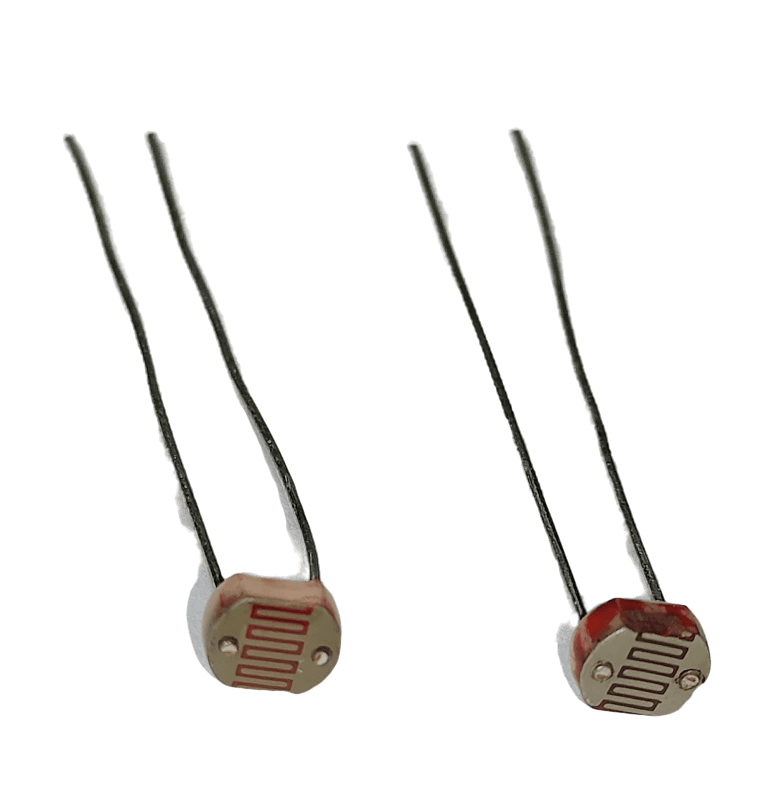
\includegraphics[scale=0.10]{electronics/fot2}
   \captionof{figure}{Fotorresistor.}
   \label{fig:fotoresistor}
\end{center}


\subsection{Joystick analógico}
El módulo de joystick analógico \cite{analog_joystick_datasheet} está construido sobre el montaje de dos potenciómetros en un ángulo de 90 grados. Los potenciómetros están conectados a una palanca corta centrada por resortes.
Este módulo produce una salida de alrededor de 2,5 V cuando la palanca se encuentra en reposo (en el centro), mientras que al desplazarse hará que la salida varíe de 0 a 5 V dependiendo de su posición. La obtención de los valores en Volts se obtiene tras convertir las lecturas en niveles lógicos mediante el módulo ADC (conversor analógico digital) \cite{ESP32_adc} del microcontrolador ESP32. En la figura \ref{fig:joystick} se puede apreciar una imagen del componente.

\begin{center}
   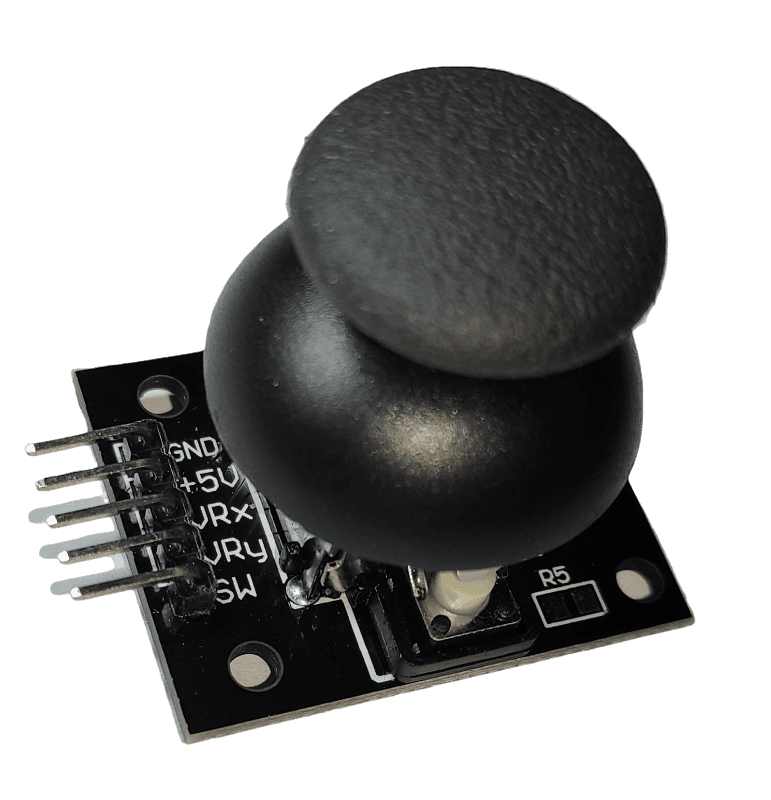
\includegraphics[scale=0.10]{electronics/joystick2}
   \captionof{figure}{Joystick analógico.}
   \label{fig:joystick}
\end{center}


\subsection{Display LCM1602A}
El display LCM1602A \cite{LCM1602A_datasheet} consta de una pantalla de cristal líquido que permite representar dos filas con hasta 16 caracteres alfanuméricos en cada una y dado que se encuentra integrada a una interfaz adaptadora I2C puede ser controlada por este protocolo. En la figura \ref{fig:display} se puede apreciar una imagen del componente.

\begin{center}
   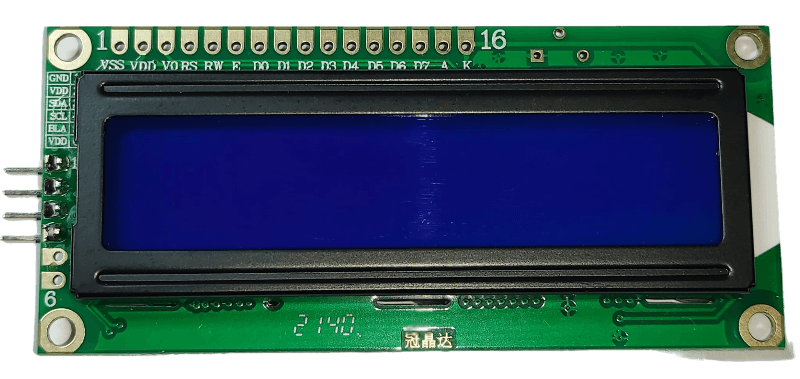
\includegraphics[scale=0.20]{electronics/display2}
   \captionof{figure}{Display LCM1602A.}
   \label{fig:display}
\end{center}

\subsection{Motores de corriente continua}
El motor DC (corriente continua) \cite{dc_motor_datasheet} es un electromotor que transforma energía eléctrica en energía mecánica. Estos motores operan con una tensión entre 3 y 6 V, corriente de 150 mA, permiten una velocidad de entre 90 y 200 RPM y un torque de entre 0,15 Nm y 0,60 Nm. En la figura \ref{fig:dc_motors} se puede apreciar una imagen del componente.


%\begin{figure}[htbp]
%\centering
\begin{center}
 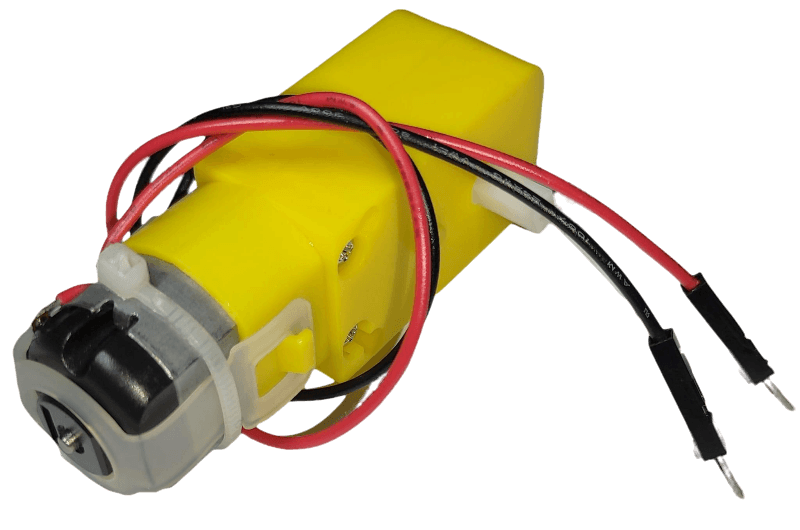
\includegraphics[scale=0.13]{electronics/engine2}
   \captionof{figure}{Motor de corriente continua.}
   \label{fig:dc_motors}
\end{center}
 %\end{figure}


\subsection{Módulos L298N}
Los módulos L298N son controladores de motores de puente H duales muy utilizados en proyectos de robótica y automoción para controlar motores de corriente continua (DC) y motores paso a paso. El módulo se basa en el IC L298N, que es un controlador de motor de doble puente H fabricado por STMicroelectronics. Este módulo posee dos puentes H que permiten controlar 2 motores DC o un motor paso a paso bipolar/unipolar. El módulo permite controlar el sentido de giro y velocidad mediante señales TTL (\textit{transistor-transistor logic}) que se pueden obtener de microcontroladores. Tiene integrado un regulador de tensión de 5 V encargado de alimentar la parte lógica del L298N cuya configuración se hace a través de un Jumper y se puede usar para alimentar el microcontrolador.

\begin{center}
  \centering
  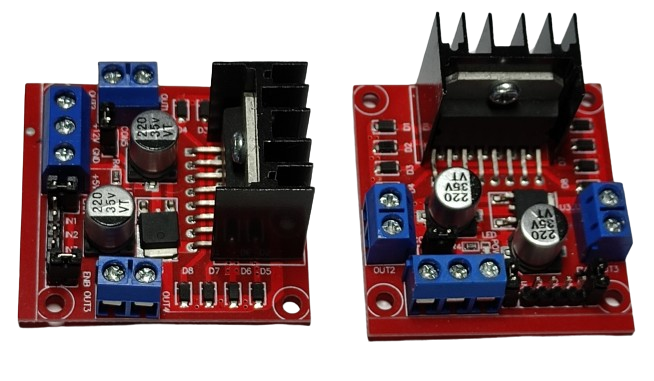
\includegraphics[scale=0.25]{electronics/l298n}
  \captionof{figure}{Interruptores de On-Off.}
  \label{fig:l298n}
\end{center}

\subsection{Pilas de Li-Ion 3,7 V}
Las pilas 18650 de 3000 mAh son baterías recargables que utilizan tecnología de iones de litio y se emplean comúnmente en una variedad de dispositivos electrónicos, como por ejemplo linternas de alta potencia, laptops, vehículos eléctricos (como bicicletas y scooters), etc. Las baterías de iones de litio son conocidas por su alta densidad de energía, su baja tasa de autodescarga y su larga vida útil en comparación con otras tecnologías de baterías recargables. Con 3000 mAh (miliamperios-hora), estas baterías ofrecen una duración prolongada, lo que es ideal para dispositivos que requieren mucha energía. Al ser recargables, son más ecológicas y económicas a largo plazo en comparación con las baterías desechables. Además, son generalmente seguras y tienen una buena estabilidad térmica, reduciendo el riesgo de explosiones o incendios.

\begin{center}
  \centering
  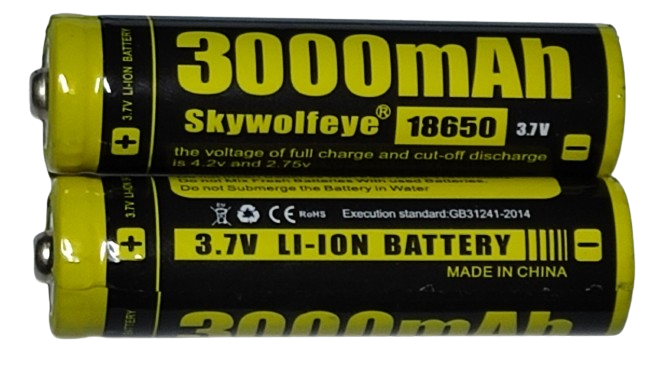
\includegraphics[scale=0.2]{electronics/baterias_liion}
  \captionof{figure}{Baterias Li-Ion.}
  \label{fig:baterias_liion}
\end{center}

\subsection{Baterías AA 1,5 V}

Las pilas AA de 1,5 V con 2600 mWh son baterías de tamaño AA que proporcionan una tensión de 1,5 V y tienen una capacidad energética de 2600 mWh. Ofrecen alta capacidad  pudiendo durar más tiempo entre recargas o reemplazos en comparación con las baterías de menor capacidad, y versatilidad, ya que al ser AA son compatibles con la mayoría de los dispositivos electrónicos que requieren alimentación de bajo voltaje.
Las pilas AA de 1,5 V con una alta capacidad como 2600 mWh son ideales para dispositivos que requieren un mayor consumo de energía, tales como cámaras digitales, linternas, juguetes electrónicos, mandos a distancia, controles de videojuegos, etc.
\begin{center}
  \centering
  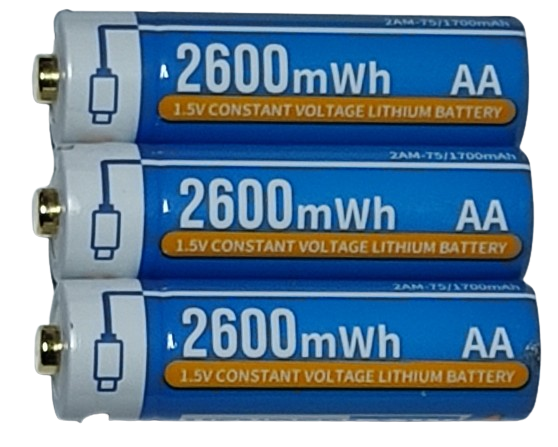
\includegraphics[scale=0.2]{electronics/pilasAA}
  \captionof{figure}{Baterías AA.}
  \label{fig:pilasAA}
\end{center}


\subsection{Plaquetas genéricas PCB}
Las plaquetas electrónicas genéricas del tipo PCB (\textit{Printed Circuit Board}), también conocidas como placas de desarrollo, son herramientas utilizadas principalmente en la educación, el diseño y el prototipado de circuitos electrónicos que constan de material aislante con patrones de cobre en una o ambas caras, donde se pueden soldar componentes para crear circuitos permanentes. Permiten el montaje de circuitos electrónicos de manera más duradera y fiable que el uso de un Protoboard y son asequibles de forma online a un bajo costo.

\begin{center}
  \centering
  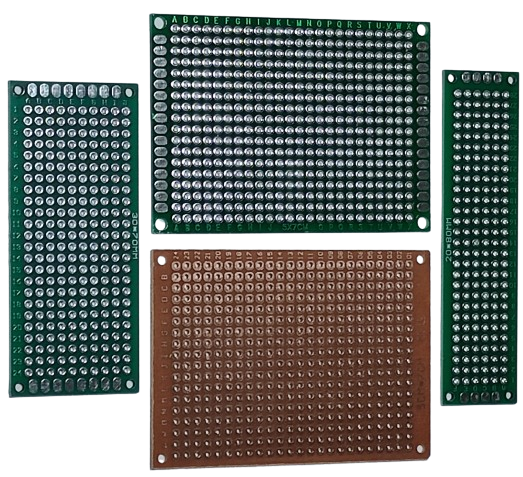
\includegraphics[scale=0.25]{electronics/plaquetas_genericas}
  \captionof{figure}{Plaquetas genéricas.}
  \label{fig:plaquetas_genericas}
\end{center}


\subsection{Cables de conexión DuPont}
Los cables Dupont son cables de conexión eléctrica utilizados comúnmente en prototipado y proyectos de electrónica. Estos cables son muy populares en la comunidad de los entusiastas y estudiantes de electrónica debido a su facilidad de uso y versatilidad. Están hechos de hilos de cobre con una cubierta de plástico aislante. Los conectores suelen ser de metal chapado para asegurar una buena conductividad. Los hay del tipo Hembra-Hembra, Hembra-Macho y Macho-Macho. Entre sus usos más comunes se encuentran la conexión de dispositivos en Protoboard sin necesidad de soldadura y la interconexión entre sensores, actuadores y terminales en pines o bahías de plaquetas impresas.

\begin{center}
  \centering
  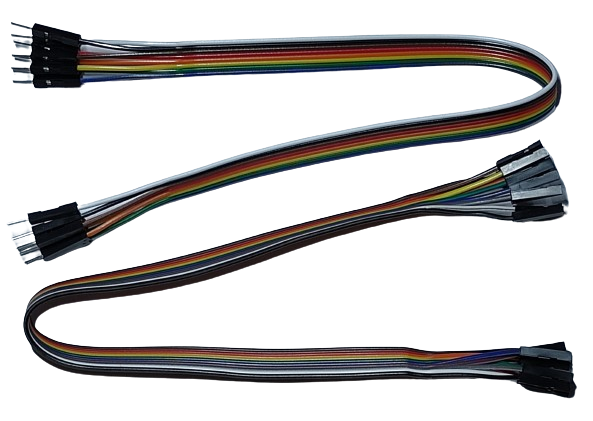
\includegraphics[scale=0.25]{electronics/dupont}
  \captionof{figure}{Cables DuPont.}
  \label{fig:dupont}
\end{center}

\subsection{Board Pin Headers para montaje de componentes y cables}
Los pines de cabecera son componentes electrónicos que consisten en filas de pines metálicos montados en una base plástica. Estos pines se utilizan para realizar conexiones eléctricas entre diferentes componentes y placas en proyectos electrónicos. La cantidad de pines puede variar en número, desde unos pocos pines hasta decenas, dependiendo de las necesidades del proyecto. Pueden encontrarse en varias configuraciones, como ser \textit{Single Row} (una sola fila de pines), \textit{Double Row} (dos filas de pines), que aumentan la capacidad de conexión en un espacio compacto, y \textit{Right Angle} (pines que se extienden en ángulo recto respecto a la base, útiles para conexiones horizontales).

\begin{center}
  \centering
  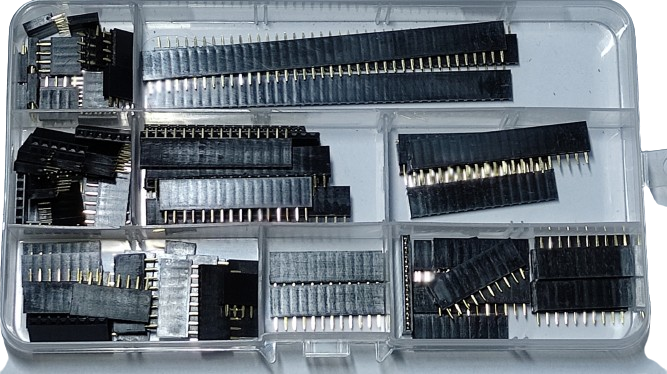
\includegraphics[scale=0.2]{electronics/pines}
  \captionof{figure}{Pines.}
  \label{fig:pines}
\end{center}

\subsection{Interruptores de On-Off}
Los interruptores de encendido-apagado (on-off) son componentes fundamentales en circuitos electrónicos que permiten controlar el flujo de corriente eléctrica. Son utilizados para conectar o desconectar la corriente en un circuito, funcionando como un medio sencillo y efectivo para gestionar la energía de dispositivos electrónicos. Se los puede encontrar en diferentes tipos, como por ejemplo, \textit{Rocker Switches} (interruptores basculantes que se operan basculando de una posición a otra), \textit{Slide Switches} (interruptores deslizantes que se operan deslizando un pequeño botón a lo largo de una pista), \textit{Toggle Switches} (interruptores de palanca que utilizan una palanca que se mueve hacia arriba y hacia abajo para cambiar entre las posiciones on y off) y \textit{Push-Button Switches} (interruptores de pulsador que al presionar el botón se conecta o desconecta el circuito).

\begin{center}
  \centering
  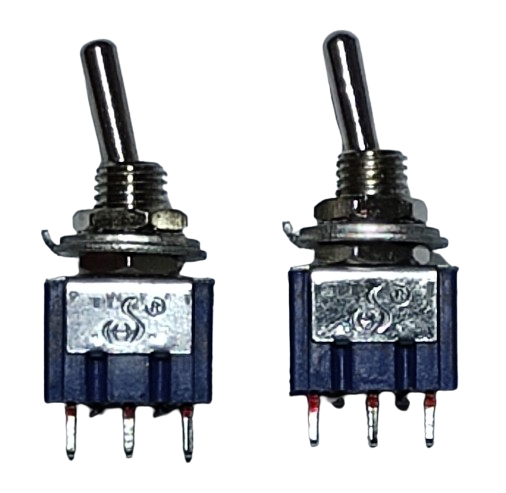
\includegraphics[scale=0.2]{electronics/interruptores}
  \captionof{figure}{Interruptores de On-Off.}
  \label{fig:interruptores}
\end{center}

\subsection{Portapilas}

Los portapilas son componentes diseñados para alojar y conectar baterías en un circuito electrónico. Estos dispositivos, generalmente hechos de plástico resistente con contactos metálicos (normalmente de níquel o acero) para asegurar una buena conductividad, facilitan la instalación y el reemplazo de baterías, asegurando una conexión segura y confiable. Se los puede encontrar comúnmente para los tipos de pilas y baterías más utilizadas, como por ejemplo AA, AAA, 9 V, 18650, CR2032, etc. Además, suelen venir en tres posibles configuraciones, un solo compartimento (para una sola batería), múltiples compartimentos (para conectar varias baterías en serie o en paralelo), y con interruptor (algunos portapilas incluyen un interruptor para encender o apagar la conexión de las baterías al circuito).

\begin{center}
  \centering
  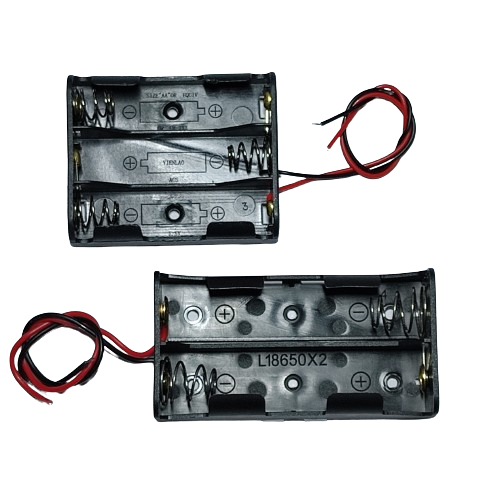
\includegraphics[scale=0.3]{electronics/porta_pilas}
  \captionof{figure}{Portapilas.}
  \label{fig:porta_pilas}
\end{center}

\subsection{Ruedas}

Las ruedas de plástico son componentes genéricos utilizados en la comunidad hobbista y estudiantil de electrónica para el armado de sistemas con desplazamiento. Se las puede comprar online a un bajo costo, usualmente vienen en kit de dos o cuatro unidades, y son compatibles con los motores de DC utilizados para moverlas.

\begin{center}
  \centering
  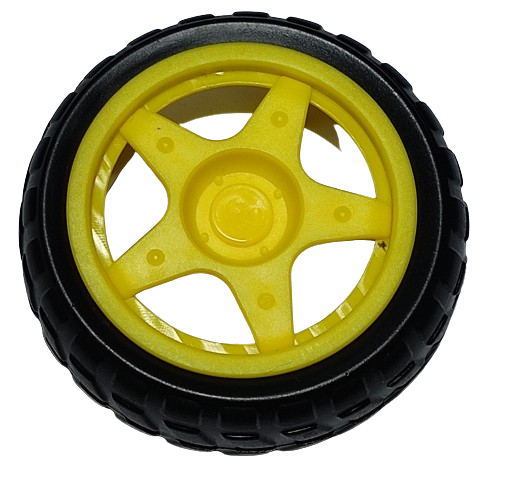
\includegraphics[scale=0.2]{electronics/ruedas}
  \captionof{figure}{Ruedas.}
  \label{fig:ruedas}
\end{center}

\subsection{Anemómetro digital}

Para la validación de los parámetros ambientales medidos por el robot se utilizó un dispositivo anemómetro digital AOPUTTRIVER AP-007-WM capaz de medir presión, temperatura y humedad ambiental, y de esta manera poder comparar los valores medidos. En la siguiente figura puede apreciarse una imagen del mismo.

\begin{center}
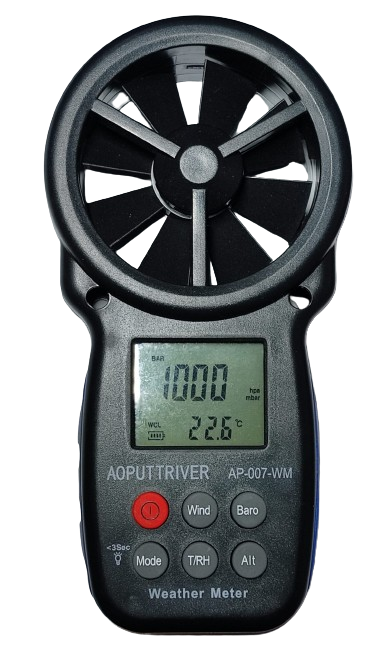
\includegraphics[scale=0.3]{electronics/anemometro}
  \captionof{figure}{Anemometro digital AOPUTTRIVER AP-007-WM.}
  \label{fig:anemometro}
\end{center}


\section{Tecnologías de software utilizadas}

\subsection{Marco de trabajo ESP-IDF}

\textit{Espressif Systems} proporciona recursos básicos de hardware y software para ayudar a los desarrolladores de aplicaciones a realizar sus ideas utilizando el hardware de la serie ESP32. El framework de software de Espressif está destinado al desarrollo de aplicaciones de IoT (Internet de las cosas) con Wi-Fi, Bluetooth, administración de energía y varias otras características del sistema.
Sus componentes son:
\begin{enumerate}
	\item Toolchain, utilizado para compilar el código para ESP32.
	\item Build tools, que provee utilidades como CMake \cite{cmake_website} y Ninja \cite{ninja_website} para construir la aplicación completa para ESP32.
	\item ESP-IDF \cite{ESPIDF_home}, que brinda la API de desarrollo para ESP32 y scripts para ejecutar Toolchain.
	
\end{enumerate}

Además de las herramientas mencionadas se utilizó el conjunto de bibliotecas y drivers provistos por el proyecto ESP-IDF-Lib \cite{esp_idf_lib_website} basados en el framework ESP-IDF.

En la figura \ref{fig:esp-idf} se puede apreciar una imagen del proceso de desarrollo y despliegue usando el framework ESP-IDF.

\begin{figure}[h]
  \centering
  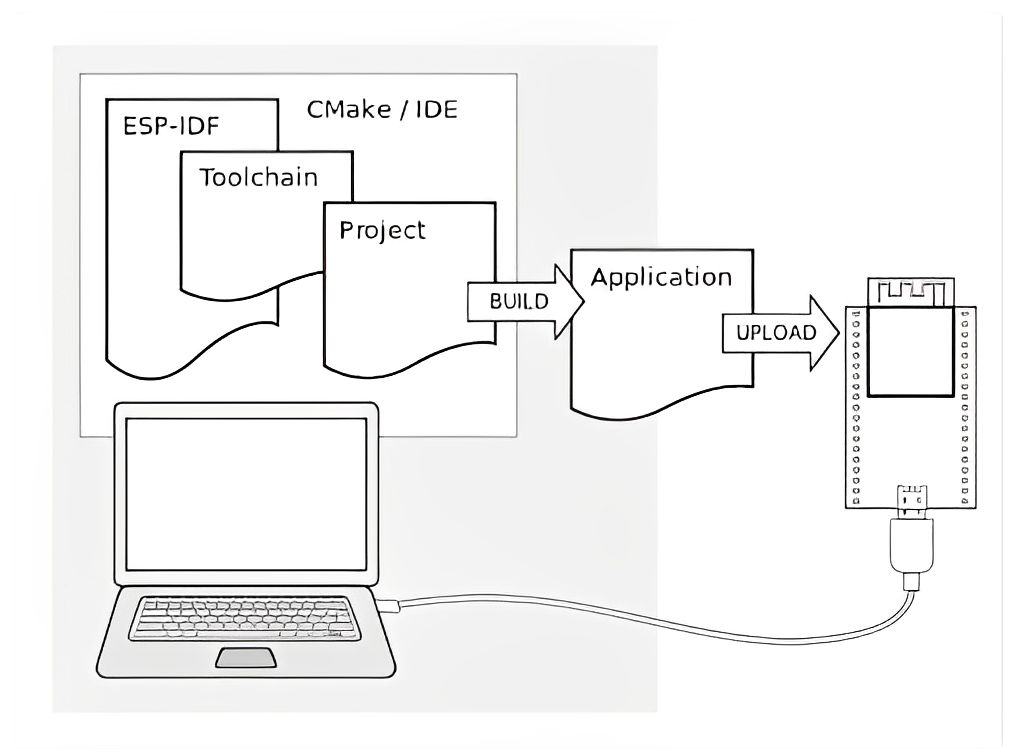
\includegraphics[scale=0.25]{conceptual/esp-idf-2}
  \caption{Proceso de desarrollo utilizando ESP-IDF\protect\footnotemark.}
  \label{fig:esp-idf}
\end{figure}

%\begin{center}
%\end{center}
%
\includegraphics[scale=0.25]{espressif}

\footnotetext{Imagen tomada de \cite{espressif-website-esp-idf}}
\subsection{Plataforma Docker}

Docker \cite{docker_website} es un proyecto de código abierto que automatiza el despliegue de aplicaciones dentro de contenedores de software, proporcionando una capa adicional de abstracción y automatización de virtualización de aplicaciones en múltiples sistemas operativos. Docker utiliza características de aislamiento de recursos del kernel Linux, tales como cgroups y espacios de nombres (namespaces) para permitir que contenedores livianos independientes se ejecuten en paralelo de manera aislada evitando la sobrecarga de iniciar y mantener máquinas virtuales.

%
\includegraphics[scale=0.15]{docker}
\subsection{Visual Studio Code}

Visual Studio Code \cite{vscode_website} es un editor de código fuente desarrollado por Microsoft para Windows, Linux, macOS y Web. Incluye soporte para la depuración, control integrado de Git, resaltado de sintaxis, finalización inteligente de código, fragmentos y refactorización de código.

%
\includegraphics[scale=0.15]{vscode}

\subsection{Sistema operativo Ubuntu}
Ubuntu \cite{ubuntu_website} es una distribución Linux basada en Debian GNU/Linux y patrocinado por Canonical, que incluye principalmente software libre y de código abierto. Puede utilizarse en ordenadores y servidores, está orientado al usuario promedio, con un fuerte enfoque en la facilidad de uso y en mejorar la experiencia del usuario.

%
\includegraphics[scale=0.25]{ubuntu}







